\subsubsection{Overview}
\label{Spike Detector}
\index{Spike Detector}\index{utilities, Spike Detector}

\begin{figure}[h]
\begin{center}
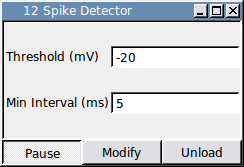
\includegraphics[width=2in]{spikedetector.png} 
\caption[Spike Detector]{The spike detector monitors the spike 
'state' based on user-defined parameters.} 
\end{center}
\label{spikedetector}
\end{figure}

This module uses a simple threshold to detect spikes. The cell can be in one of 5 states:
\begin{description}
 \item[0] Looking for voltage to cross above threshold
 \item[1] Cell has crossed threshold going up
 \item[2] Cell is above threshold
 \item[3] Cell is crossing threshold going down
 \item[4] Depolarization block. cell has been above threshold for more than 100ms
 \item[-1] Reset state. Will reset if cell hasn’t spike since the minimum interval
\end{description}

In addition, you can set a refractory period, the minimum interval that must go by before another spike can be detected again.

\subsubsection{Input Channels}
\begin{description}
\item[input(0)- "Vm" (mV)] the membrane potential
\end{description}

\subsubsection{Output Channels}
\begin{description}
\item[output(0) - "Spike State"] see description above
\end{description}

\subsubsection{Parameters}
\begin{description}
\item[Threshold (mV)] the threshold at which a spike is detected
\item[Min. Interval (ms)] minimum interval (refractory period) that must pass before another spike can be detected
\end{description}